% !TeX program = xelatex
% !TeX spellcheck = sl_SI
% Na osnovi predlog LADISK (Martin Česnik, Janko Slavič), posodobitev 2026.
\documentclass[12pt,a4paper,twoside,openright,fleqn]{book}
% Oblikovanje po Wordovi predlogi FS, september 2026.
\usepackage{iftex}
\ifPDFTeX
  \PackageError{FS2026}{Uporabite XeLaTeX ali LuaLaTeX}{Pisava Times New Roman zahteva XeLaTeX ali LuaLaTeX.}
\fi
\usepackage{fontspec}
\setmainfont{Times New Roman}
\setmonofont{Latin Modern Mono}[Scale=MatchLowercase]
\usepackage[english,slovene]{babel}
\usepackage{amsmath,amssymb,bm}
\usepackage{graphicx}
\usepackage[section]{placeins}
\usepackage{float}
\usepackage{enumitem}
\usepackage{longtable,booktabs,array}
\usepackage{fancyhdr}
\usepackage{tocloft}
\usepackage{titlesec}
\usepackage{pdfpages}
\usepackage{pdflscape}
\usepackage{caption,subcaption}
\usepackage{icomma}
\usepackage{etoolbox}
\usepackage{notoccite}
\usepackage[numbers,square,sort&compress]{natbib}
\usepackage[inner=30mm,outer=25mm,top=30mm,bottom=25mm,headheight=15pt]{geometry}
\usepackage[unicode,hidelinks]{hyperref}

% Umerjeno po dejanskem razmiku osnovnic v Wordovem PDF-ju (pribl. 15,9 bp).
% Times New Roman ima v XeLaTeXu drugačne metrike, zato faktor ni neposredno 1,15.
\linespread{1.10}
\setlength{\parindent}{0pt}
% Sosednja odmika Wordovih odstavkov po 8 pt se ne seštevata.
\setlength{\parskip}{8pt}
\raggedbottom
\setlength{\emergencystretch}{1em}
\setlength{\mathindent}{5mm}
\setcounter{secnumdepth}{2}
\setcounter{tocdepth}{2}
\setlist[itemize,1]{label=\textbullet,leftmargin=7.5mm,itemsep=2pt,parsep=0pt,topsep=2pt}
\setlist[itemize,2]{label=\(\circ\),leftmargin=7.5mm,itemsep=8pt,parsep=0pt,topsep=2pt}
\setlist[enumerate]{leftmargin=*,itemsep=2pt,parsep=0pt}
\DeclareCaptionFont{fsfont}{\fontsize{11}{12.65}\selectfont}
\captionsetup{font=fsfont,labelsep=colon}
\captionsetup[table]{position=top,justification=raggedright,singlelinecheck=false,skip=4pt}
\captionsetup[figure]{position=bottom,justification=centering,skip=4pt}
\captionsetup[subfigure]{labelfont=normalfont}
% \@floatboxreset znotraj plavajočega okolja kliče \normalsize, zato velikost
% pisave v preglednicah nastavimo za njim (\AtBeginEnvironment{table} ne deluje)
\makeatletter
\appto\@floatboxreset{\ifdefstring{\@captype}{table}{\fontsize{10}{11.5}\selectfont}{}}
\makeatother
\addto\captionsslovene{\renewcommand{\tablename}{Preglednica}\renewcommand{\bibname}{Literatura}}
\setlength{\textfloatsep}{12pt}
\setlength{\intextsep}{12pt}
\newcommand{\minitab}[2][l]{\begin{tabular}{#1}#2\end{tabular}}
\renewcommand{\thetable}{\thechapter.\arabic{table}}
\renewcommand{\thefigure}{\thechapter.\arabic{figure}}
\renewcommand{\theequation}{\thechapter.\arabic{equation}}

\titleformat{\chapter}[hang]{\fontsize{24}{27.6}\selectfont\bfseries}{\thechapter}{1em}{}
\titleformat{name=\chapter,numberless}[hang]{\fontsize{24}{27.6}\selectfont\bfseries}{}{0pt}{}
% Odmiki so umerjeni po prvi oštevilčeni strani Wordove predloge.
\titlespacing*{\chapter}{0pt}{111pt}{36pt}
\titleformat{\section}{\fontsize{18}{20.7}\selectfont\bfseries}{\thesection}{1em}{}
\titlespacing*{\section}{0pt}{15.25pt}{6pt}
\titleformat{\subsection}{\fontsize{14}{16.1}\selectfont\bfseries}{\thesubsection}{1em}{}
\titlespacing*{\subsection}{0pt}{18pt}{6pt}
\titleformat{\subsubsection}{\normalsize\bfseries}{}{0pt}{}
\titlespacing*{\subsubsection}{0pt}{12pt}{3pt}
\renewcommand{\cftchapdotsep}{\cftdotsep}
% Naslovi prve ravni (\chapter) so v kazalu veliki 16 pt.
\renewcommand{\cftchapfont}{\fontsize{16}{19.27}\selectfont\bfseries}
\renewcommand{\cftchappagefont}{\fontsize{16}{19.27}\selectfont\bfseries}
% Naslovi druge ravni (\section) so v kazalu izpisani krepko.
\renewcommand{\cftsecfont}{\bfseries}
\renewcommand{\cftsecpagefont}{\bfseries}
% Navpični razmiki v kazalu so umerjeni po Wordovi predlogi (razmiki osnovnic:
% poglavje-poglavje 29,2 pt, poglavje-razdelek 27,5 pt, razdelek-razdelek 26 pt,
% razdelek-podrazdelek 21,8 pt). Odstavek vpisa poglavja se konča v njegovi
% pisavi, da velja razmik vrstic 16-pt pisave; kern za vpisom ne vpliva na \addvspace.
\setlength{\cftbeforechapskip}{6.3pt}
\setlength{\cftbeforesecskip}{10.1pt}
\setlength{\cftbeforesubsecskip}{5.9pt}
\renewcommand{\cftchapafterpnum}{\fontsize{16}{19.27}\selectfont\par\kern1.7pt}

\fancypagestyle{fancy_nohead}{%
  \fancyhf{}\fancyfoot[LE,RO]{\thepage}
  \renewcommand{\headrulewidth}{0pt}\renewcommand{\footrulewidth}{0pt}}
\fancypagestyle{plain}{%
  \fancyhf{}\fancyfoot[LE,RO]{\thepage}
  \renewcommand{\headrulewidth}{0pt}}
\renewcommand{\chaptermark}[1]{\markboth{#1}{}}
\fancypagestyle{vsebina}{%
  \fancyhf{}
  \fancyhead[LE,RO]{\nouppercase{\leftmark}}
  \fancyfoot[LE,RO]{\thepage}
  \renewcommand{\headrulewidth}{0.1mm}
  \renewcommand{\footrulewidth}{0pt}}

% Povsem prazna stran brez številke in glave (npr. vezni list).
\newcommand{\praznastran}{\null\thispagestyle{empty}\newpage}
\makeatletter
% Soda prazna stran pred novim poglavjem ima, kot v Wordu, številko in glavo
% trenutnega sloga strani (na naslovnih straneh je slog empty).
\renewcommand{\cleardoublepage}{\clearpage\if@twoside\ifodd\c@page\else\null\newpage\fi\fi}
\newcommand{\vsebinskokazalo}{\begingroup\setlength{\parskip}{0pt}\@starttoc{toc}\endgroup}
\makeatother
% Združljivost s starimi poglavji; novih ročnih praznih strani ni treba dodajati.
\newcommand{\addifeven}{\cleardoublepage}

% Formalni naslovi na vrhu strani; samo seznama se vpišeta v kazalo.
\newcommand{\predpoglavje}[1]{%
  \cleardoublepage\thispagestyle{fancy_nohead}\markboth{#1}{}
  % Umerjeno po Wordu: osnovnica naslova 104 pt od vrha strani, zgornji rob
  % črte 7,8 pt pod osnovnico (neodvisno od spodnjih zank črk), prva vrstica
  % besedila 35,6 pt pod črto.
  \vspace*{-23.6pt}{\fontsize{18}{20.7}\selectfont\bfseries\raggedright\hyphenpenalty=10000 #1\par}
  \nobreak\vskip-\prevdepth\vskip7.6pt\hrule height 0.4pt\nobreak\vspace{19.2pt}}
\newcommand{\predpoglavjevkazalu}[1]{%
  \predpoglavje{#1}\phantomsection\addcontentsline{toc}{chapter}{\protect\brezzamika #1}}
% Neoštevilčeni vpisi v kazalu nimajo visečega zamika druge vrstice (kot v Wordu).
% Ukaz ponastavi levi zamik (globalno, ker je vpis v skupini; privzeta vrednost
% je tako in tako 0) in izravna začetni odmik tocloft.
\newcommand{\brezzamika}{\global\leftskip=\cftchapindent\relax\hskip\cftchapnumwidth\relax}
\AtBeginDocument{\pdfstringdefDisableCommands{\let\brezzamika\relax}}
\newcounter{priloga}
\renewcommand{\thepriloga}{\Alph{priloga}}
% V doktorski predlogi so priloge oblikovane kot formalna poglavja v kazalu.
\newcommand{\priloga}[1]{%
  \stepcounter{priloga}
  \predpoglavje{Priloga \Alph{priloga} -- #1}
  \addtocounter{priloga}{-1}\refstepcounter{priloga}
  \addcontentsline{toc}{chapter}{\protect\brezzamika Priloga \Alph{priloga} -- #1}
  \markboth{Priloga \Alph{priloga}}{}
  \renewcommand{\thechapter}{\Alph{priloga}}
  \setcounter{figure}{0}\setcounter{table}{0}\setcounter{equation}{0}}
\setlength{\bibsep}{8pt}
\renewcommand{\bibfont}{\normalfont\normalsize}
\urlstyle{same}
\AtBeginDocument{\hypersetup{pdftitle={\naslovSlo},pdfauthor={\avtor},pdfsubject={\tipDela}}}

\newcommand{\poglavjeref}[1]{%
	\textbf{\ref{#1}~\nameref{#1}}%
}

% Tu izpolnite podatke vašega doktorskega dela
\newcommand{\naslovSlo}{Naslov dela}
\newcommand{\naslovAng}{Thesis title}
\newcommand{\avtor}{Ime Priimek avtorja}

\newcommand{\tipDela}{Doktorsko delo}
% Izberite obliko glede na spol kandidata oz. kandidatke.
\newcommand{\predlozil}{Predložil}
% \newcommand{\predlozil}{Predložila}

\newcommand{\mentor}{akad.~naziv Ime Priimek, izobrazba}
\newcommand{\somentor}{akad.~naziv Ime Priimek, izobrazba} % Prazno, če somentorja ni.

\newcommand{\zagovorMesec}{mesec}
\newcommand{\zagovorLeto}{leto zagovora}

% Podatki za načrt ravnanja z raziskovalnimi podatki (NRRP)
\newcommand{\doktorskiProgram}{Doktorski študijski program Strojništvo, področje \ldots}

% Podatki za generacijo strani Izvleček/Abstract
\newcommand{\UDK}{XXX.XX:XXX.(XXX.X)}

\newcommand{\tekocaStevilka}{DR III/XX} % Prepišite z odločbe o potrjeni temi.

% Navedite 5--8 ključnih besed, vsako v svoji vrstici. Slovenske ključne
% besede praviloma pišemo z malo začetnico.
\newcommand{\kljucneBesede}{%
ključna beseda 1 (vse ključne besede pišemo z malo začetnico)\\
ključna beseda 2 (zahtevanih je 5--8 ključnih besed)\\
ključna beseda 3\\
ključna beseda 4\\
ključna beseda 5\\
ključna beseda 6}

\newcommand{\izvlecek}{% Nadomestite z dejanskim izvlečkom (praviloma 150--300 besed, do pol strani).
V začetku izvlečka je jedrnat opis obravnavanega problema. Sledi opis izbrane metodologije in nato opis najpomembnejših rezultatov oz. ugotovitev brez dodatnih pojasnjevanj. Obseg izvlečka je praviloma omejen na 150 do 300 besed oziroma naj ne presega polovice strani. Študent pridobi UDK številko v knjižnici FS, za katero mora zaprositi vsaj 3 delovne dni pred oddajo. To lahko naredi na podlagi navedenih ključnih besed in povzetka, ki jih mora študent poslati v knjižnico na naslov knjiznica@fs.uni-lj.si. Kandidat mora vnesti tudi tekočo številko doktorskega dela, naslov dela, svoje ime in priimek ter ključne besede.}

\newcommand{\keywords}{%
keyword 1 (write all keywords in lower case)\\
keyword 2 (five to eight keywords are required)\\
keyword 3\\
keyword 4\\
keyword 5\\
keyword 6}

\newcommand{\abstract}{%
At the beginning of the abstract, a concise description of the addressed problem must be provided. This is followed by a description of the chosen methodology and then by a presentation of the most important results or findings, without additional explanations. The abstract should generally be limited to 150 to 300 words and should not exceed half a page. The candidate must enter the UDC number, which is obtained from the library based on the submitted information about the thesis: the title, the supervisor and any co-supervisors, at least five keywords, and the abstract. The candidate must also enter the serial number of the thesis, the title of the work, their name and surname, and the keywords. Keywords are generally written in the plural.}

\newcommand{\datotekaTeme}{tema.pdf} % Odločba o potrjeni temi; vključijo se vse strani PDF.

\newif\ifzahvala

\zahvalatrue % Za izpust zahvale uporabite \zahvalafalse.


\begin{document}
% Platnica, njena prazna hrbtna stran in prazen vezni list.
\pagestyle{empty}
\hypersetup{pageanchor=false}
% ta stran se zgenerira sama, za vhodne podatke uporabite podatki.tex

\thispagestyle{empty}
\AddToHookNext{shipout/foreground}{%
  \begingroup
  \linespread{1}\selectfont
  \setlength{\parindent}{0pt}
  \setlength{\parskip}{0pt}
  % Višina osnovnice, velikost pisave, razmik vrstic, besedilo.
  \newcommand{\platnicaPolje}[4]{%
    \put(88.5bp,-#1bp){%
      \parbox[t]{155mm}{\centering
        \fontsize{#2bp}{#3bp}\selectfont #4\par}}}
  
  \platnicaPolje{98}{14}{18.6}{\textbf{UNIVERZA V LJUBLJANI}}
  \platnicaPolje{130}{14}{18.6}{Fakulteta za strojništvo}
  \platnicaPolje{319}{20}{26.5}{\textbf{\naslovSlo}}
  \platnicaPolje{413}{14}{18.6}{\tipDela}
  \platnicaPolje{469.5}{14}{18.5}{\predlozil{} Fakulteti za strojništvo Univerze v~Ljubljani za pridobitev znanstvenega naslova doktor znanosti}
  \platnicaPolje{566.5}{16}{21.2}{\textbf{\avtor}}
  \platnicaPolje{753}{14}{18.6}{Ljubljana, \zagovorMesec~\zagovorLeto}
  \endgroup
}
\null


\clearpage
\praznastran
\praznastran
\praznastran

% Štetje formalnih strani se začne z notranjo naslovnico (i).
\pagenumbering{roman}
\hypersetup{pageanchor=true}
% ta stran se zgenerira sama, za vhodne podatke uporabite podatki.tex


\thispagestyle{empty}
\AddToHookNext{shipout/foreground}{%
	\begingroup
	\linespread{1}\selectfont
	\setlength{\parindent}{0pt}
	\setlength{\parskip}{0pt}
	% Višina osnovnice, velikost pisave, razmik vrstic, besedilo.
	\newcommand{\platnicaPolje}[4]{%
		\put(88.5bp,-#1bp){%
			\parbox[t]{155mm}{\centering
				\fontsize{#2bp}{#3bp}\selectfont #4\par}}}
	
	\platnicaPolje{98}{14}{18.6}{\textbf{UNIVERZA V LJUBLJANI}}
	\platnicaPolje{130}{14}{18.6}{Fakulteta za strojništvo}
	\platnicaPolje{319}{20}{26.5}{\textbf{\naslovSlo}}
	\platnicaPolje{392.4}{14}{18.6}{\tipDela}
	\platnicaPolje{455.3}{14}{18.5}{\predlozil{} Fakulteti za strojništvo Univerze v~Ljubljani za pridobitev znanstvenega naslova doktor znanosti}
	\platnicaPolje{577.8}{16}{21.2}{\textbf{\avtor}}
	\platnicaPolje{665.1}{14}{18.5}{Mentor: \mentor
	\par \if\relax\detokenize\expandafter{\somentor}\relax\else
	Somentor: \somentor\par
	\fi}
	\platnicaPolje{767.1}{14}{18.6}{Ljubljana, \zagovorMesec~\zagovorLeto}
	\endgroup
}
\null


\cleardoublepage

\IfFileExists{\datotekaTeme}{%
  \includepdf[pages=-,pagecommand={\thispagestyle{empty}}]{\datotekaTeme}
}{%
  \thispagestyle{empty}
  [Prostor za odločbo o potrjeni temi doktorskega dela s strani UL. Datoteko
  \texttt{tema.pdf} shranite ob glavni datoteki \texttt{predloga.tex}.]
  \clearpage}

\cleardoublepage

\pagestyle{fancy_nohead}

\ifzahvala\predpoglavje{Zahvala}

Pisanje zahvale ali posvetila je neobvezno. Pri zahvali napišite zahvalo tistim, ki so pomagali pri nastanku dela in brez katerih delo ne bi nastalo v takšni obliki, kot je. Navadno se je potrebno zahvaliti v prvi vrsti mentorju, somentorju in inštituciji, ki je morda finančno ali kako drugače podprla izvedbo doktorskega dela. Nato sledijo asistenti, ostali sodelavci in vaši kolegi, ki so pomagali pri teoretičnem in eksperimentalnem delu. Na koncu se po navadi zahvalimo še družini.
\fi
% ta stran se zgenerira sama, za vhodne podatke uporabite podatki.tex

\predpoglavje{Izvleček}
\noindent\hfill UDK \UDK\par
Tek. štev.: \tekocaStevilka\par
\vspace{16pt}

{\fontsize{14}{16.1}\selectfont\bfseries \naslovSlo\par}
\vspace{16pt}

\avtor\par
\vspace{16pt}

\noindent\begin{tabular}{@{}p{35mm}@{}p{\dimexpr\textwidth-35mm\relax}@{}}
Ključne besede: & \parbox[t]{\linewidth}{%
  \linespread{1}\fontsize{12pt}{20.7bp}\selectfont\kljucneBesede}
\end{tabular}\par
\vspace{24pt}
 \izvlecek


\predpoglavje{Abstract}
\begin{otherlanguage}{english}
\noindent\hfill UDC \UDK\par
No.: \tekocaStevilka\par
\vspace{16pt}

{\fontsize{14}{16.1}\selectfont\bfseries \naslovAng\par}
\vspace{16pt}

\avtor\par
\vspace{16pt}

\noindent\begin{tabular}{@{}p{35mm}@{}p{\dimexpr\textwidth-35mm\relax}@{}}
Keywords: & \parbox[t]{\linewidth}{%
  \linespread{1}\fontsize{12pt}{20.7bp}\selectfont\keywords}
\end{tabular}\par
\vspace{24pt}
\abstract
\end{otherlanguage}

\predpoglavje{Kazalo}
% Razmik med naslovom in prvim vpisom je v Wordu za 13 pt večji kot pri drugih
% formalnih naslovih.
\vspace*{12.2pt}
\vsebinskokazalo


\predpoglavjevkazalu{Seznam uporabljenih simbolov}
% Glava preglednice je v Wordu 38 pt pod črto naslova (pri besedilu 35,6 pt).
\setlength{\LTpre}{3.3pt}
% Ločite latinske in grške simbole
% Enote so pokončne, skalarne veličine poševne, vektorji krepko poševni.
\begin{longtable}[l]{@{}p{22mm}p{28mm}p{\dimexpr\textwidth-50mm-4\tabcolsep\relax}@{}}
\toprule
Oznaka & Enota & Pomen\\ \midrule
\endfirsthead
\multicolumn{3}{l}{nadaljevanje}\\
\toprule Oznaka & Enota & Pomen\\ \midrule
\endhead
\multicolumn{3}{r}{se nadaljuje}\\
\endfoot
\endlastfoot
\multicolumn{3}{@{}l}{~}\\
$A$ & $\mathrm{m^2}$ & površina\\
$C$ & $/$ & koncentracija\\
$D$ & $\mathrm{m^2\,s^{-1}}$ & difuzijski koeficient\\
$d$ & $\mathrm{mm}$ & premer\\
$P$ & $\mathrm{Pa,\ bar}$ & tlak\\
$V$ & $\mathrm{m^3}$ & volumen\\
$v$ & $\mathrm{m\,s^{-1}}$ & hitrost\\
\multicolumn{3}{@{}l}{~}\\
$\gamma$ & $\mathrm{m^2\,l^{-1}}$ & stopnja povečevanja mašenja\\
$\varepsilon$ & $/$ & učinkovitost\\
$\eta$ & $\mathrm{Pa\,s}$ & dinamična viskoznost\\
\multicolumn{3}{@{}l}{~}\\
\midrule
\multicolumn{3}{@{}l}{Indeksi}\\
\midrule
\multicolumn{3}{@{}l}{~}\\
$\mathrm{cel}$ & & celotni\\
$\mathrm{f}$ & & filtracija\\
$\mathrm{k}$ & & koncentrat\\
$\mathrm{p}$ & & permeat\\
$\mathrm{z}$ & & začetni\\
\end{longtable}

\predpoglavjevkazalu{Seznam uporabljenih okrajšav}
% Okrajšave razvrstite po abecedi. Pri tujih besednih zvezah navedite
% slovenski pomen in nato izvirno besedno zvezo v poševnem tisku.
\begin{longtable}[l]{@{}p{34mm}p{\dimexpr\textwidth-34mm-2\tabcolsep\relax}@{}}
\toprule
Okrajšava & Pomen\\ \midrule
\endfirsthead
\multicolumn{2}{l}{nadaljevanje}\\
\toprule Okrajšava & Pomen\\ \midrule
\endhead
\multicolumn{2}{r}{se nadaljuje}\\
\endfoot
\endlastfoot
\multicolumn{2}{@{}l}{~}\\
ACH & aluminijev klorhidrat, vrsta koagulanta\\
CODMn & ekvivalent kisika, potrebnega za oksidacijo organske vsebine vzorca z uporabo trivalentnega mangana (angl.~Chemical Oxygen Demand)\\
GAC & aktivno oglje v granulah (angl.~Granular Activated Carbon)\\
MF & Mikrofiltracija\\
NF & nanofiltracija\\
PAC & aktivno oglje v prahu (angl.~Powder Activated Carbon)\\
RO & reverzna osmoza\\
SCADA & sistem za nadzor in zajemanje podatkov (angl.~Supervisory Control And Data Acquisition)\\
TOC & skupna količina vseh organskih spojin v vzorcu (angl.~Total Organic Carbon)\\
TSS & količina vseh suspendiranih trdnih delcev v vzorcu (angl.~Total Suspended Solids)\\
UF & ultrafiltracija\\
\end{longtable}
% Privzeti odmik pred preglednicami longtable v nadaljevanju dokumenta.
\setlength{\LTpre}{\bigskipamount}


\cleardoublepage
\pagenumbering{arabic}
\pagestyle{vsebina}
\chapter{Uvod}\label{cha:uvod}
Uvodno poglavje naj vsebuje splošni opis oziroma razlago obravnavane tematike. Predstavite izhodišča doktorskega dela, problematiko in njegov pomen. V uvodu ne predstavljajte rezultatov in sklepov.

V tej predlogi je \textbf{v nevsebinskem delu} (do strani xvi) potrebno izpolniti vse informacije, da bodo ustrezale podatkom kandidata oz.~kandidatke in doktorskega dela. Kazalo vsebine se ob prevajanju osveži samodejno. Pri tem upoštevajte navodila glede uporabe ustreznih slogov, ki so navedena v \textbf{prilogi \ref{cha:priloga}}.

V tej predlogi so \textbf{v vsebinskem delu} navodila in primeri za oblikovanje doktorskega dela, tehnične podrobnosti pa so dodatno opisane v \textbf{prilogi \ref{cha:priloga}}. Celotno besedilo je potrebno nadomestiti z besedilom, ki vsebinsko ustreza doktorskemu delu.

V primeru, da je obravnavana tematika tesno povezana s širšim znanstvenim področjem oz.~poznavanjem določenih pojavov, procesov, postopkov, preračunov itn., ki jih doktorsko delo sicer ne obravnava neposredno, so pa pomembni za njegovo razumevanje, se lahko v tem poglavju predstavi omenjeno širšo tematiko.

\section{Struktura doktorskega dela}\label{sec:struktura_dela}
V tem delu se osredotočite na to, kako je delo strukturirano (po poglavjih), torej npr.~kje je predstavljen nek vsebinski sklop in kako so posamezni vsebinski sklopi med seboj povezani.

\chapter{Pregled stanja razvoja}\label{cha:pregled}
Ne glede na to, ali je delo teoretično ali eksperimentalno usmerjeno, je potrebno najprej obdelati osnove obravnavane tematike.

\section{Podpoglavja in slogi}\label{sec:podpoglavja}
To je primer teksta, ki sledi naslovu podpoglavja na 2.~ravni. Posamezne dele vsebine smiselno razdelite v podpoglavja, ki naj bodo ustrezno naslovljena in zaporedno oštevilčena (številčenje poglavij naj bo samodejno). Slog naslovov podpoglavij naj ustreza prednastavljenim stilom, ki so prikazani v tej predlogi in podrobno opisani v \textbf{prilogi \ref{cha:priloga}}.

\subsection{Podpoglavje na 3.~ravni}\label{sec_podpoglavje_3}
To je primer teksta, ki sledi naslovu podpoglavja na 3.~ravni. Poglavja na 1., 2.~in 3.~ravni so številčena in se pojavijo tudi v kazalu, kar je v predlogi že nastavljeno. Uporabite lahko največ 4 ravni naslovov, pri čemer četrta raven ni oštevilčena in se ne pojavi v kazalu.

\subsubsection{Podpoglavje na 4.~ravni}
To je primer teksta, ki sledi naslovu podpoglavja na 4. ravni. Podpoglavje na 4. ravni je neoštevilčeno in se ne pojavi v kazalu, kar je v predlogi že nastavljeno.


\section{Odstavki in naštevanje}\label{sec:odstavki}
Prve vrstice odstavkov naj ne bodo zamaknjene. Med odstavke ne vrivajte dodatnih praznih vrstic. Uporaba \textbf{krepkega tiska} v besedilu je smiselna (ni pa nujna):
\begin{itemize}
\item kadar v besedilu prvič omenimo in opredelimo zelo pomemben pojem za razumevanje dela,
\item kadar želimo posebej poudariti kakšen del ali misel,
\item kadar želimo pri naštevanju vidno ločiti posamezne dele besedila.
\end{itemize}

Kadar v besedilu uporabljamo besede iz tujih jezikov, uporabljamo poševni tisk (angl.~\emph{italic}). \underline{Podčrtanega besedila} praviloma ne uporabljamo.

\subsubsection{Ravni naštevanja}
Ne glede na to, koliko hierarhičnih ravni alinej je v besedilu uporabljenih za naštevanje (običajno ne več kot 2), v celotnem besedilu vedno uporabljamo enako kombinacijo ter način označevanja posameznih ravni alinej. S tem dosežemo poenoten videz besedila. Slog za posamezen nivo alinej je že nastavljen. 

Podrobnosti sloga za 1.~in 2.~raven naštevanja so opisane v \textbf{prilogi \ref{cha:priloga}}.
\begin{itemize}
\item primer 1.~ravni naštevanja:
\begin{itemize}
\item primer 2.~ravni naštevanja,
\item primer 2.~ravni naštevanja,
\end{itemize}
\end{itemize}
Med alineje in pred novim odstavkom besedila za zadnjo alinejo ne vstavljajte praznih vrstic.


\section{Preglednice}\label{sec:preglednice}
Preglednice naj imajo vstavljene napise z izbranim ustreznim stilom, naj bodo zaporedno oštevilčene in oblikovane, kot to opredeljujejo navodila v \textbf{prilogi \ref{cha:priloga}}. Preglednice in njihovi napisi naj bodo levo poravnani. Med besedilom pred preglednico, napisom preglednice in preglednico ne vstavljajte dodatnih praznih vrstic.

Napis preglednice naj se začne z veliko začetnico in konča s končnim ločilom, kot je to prikazano na primeru preglednice \ref{tab:ucinkovitost}. Napis naj bo dovolj poveden, da je vsebino preglednice možno razumeti kot samostojen element.

Preglednica naj bo smiselno umeščena v besedilo. Običajno preglednico umestimo pod odstavek, v katerem preglednico prvič omenimo. Če preglednico zaradi bolj tekočega oblikovanja besedila umestimo drugače, naj bo umeščena v bližini prve omembe v besedilu, vendar za prvo omembo. Pri sklicevanju na preglednice in druge dele besedila sledite navodilom, ki so opisana v \textbf{prilogi \ref{cha:priloga}}.

\begin{table}[htbp]
	\caption{Učinkovitost procesov odstranjevanja različnih onesnaževalcev vode.}\label{tab:ucinkovitost}
	\setlength{\tabcolsep}{4pt}
	\renewcommand{\arraystretch}{1.3}
\begin{tabular}{@{}>{\raggedright\arraybackslash}m{52mm}
		*{4}{>{\centering\arraybackslash}m{22mm}}@{}}
	\toprule
	\multicolumn{1}{@{}>{\centering\arraybackslash}m{52mm}}{Proces}
	& Odstranitev mikroorganizmov
	& Odstranitev suspendiranih snovi
	& Odstranitev raztopljenih anorganskih snovi
	& Odstranitev raztopljenih organskih snovi \\
	\midrule
	\textbf{Biološki} & & & & \\
	\hspace{3mm}Aktivno blato              & $+$ & $+$ & $-$ & $+$ \\
	\hspace{3mm}Anaerobna obdelava         & $-$ & $+$ & $-$ & $+$ \\
	\hspace{3mm}Biofiltri                  & $-$ & $-$ & $-$ & $+$ \\
	\addlinespace[2pt]
	\textbf{Fizikalni} & & & & \\
	\hspace{3mm}Adsorpcija na aktiv.\ oglju: & & & & \\
	\hspace{7mm}v granulah                 & $-$ & $+$ & $-$ & $+$ \\
	\hspace{7mm}v prahu                    & $+$ & $+$ & $-$ & $+$ \\
	\hspace{3mm}Konvencionalna filtracija  & $-$ & $+$ & $-$ & $-$ \\
	\hspace{3mm}Flokulacija + sediment.    & $+$ & $+$ & $-$ & $-$ \\
	\hspace{3mm}Membranski procesi & & & & \\
	\hspace{7mm}MF                         & $+$ & $+$ & $-$ & $-$ \\
	\bottomrule
\end{tabular}
{\fontsize{8}{9.6}\selectfont Legenda: $+$ odstranjevanje poteka učinkovito, o~odstranjevanje delno poteka, $-$ odstranjevanje ne poteka}
\end{table}

Če je preglednica ali del preglednice povzet iz drugega vira, ga je potrebno citirati, kot je to prikazano na primeru preglednice \ref{tab:poraba}. Če je povzeta celotna preglednica, se številko reference napiše k napisu preglednice. Če so povzete le določene vrednosti ali besedilo znotraj celic, se to lahko citira v posameznih celicah ali na koncu posamezne vrstice.

\begin{table}[htbp]
	\caption{Kumulativne vrednosti porabe vode na vseh filtracijskih enotah za leto 2012 \cite{grote2021}.}\label{tab:poraba}
	\setlength{\tabcolsep}{4pt}
	\renewcommand{\arraystretch}{1.3}
\begin{tabular*}{\textwidth}{@{\extracolsep{\fill}}l*{7}{c}@{}}
	\toprule
	& $V_\mathrm{f}$
	& $V_\mathrm{sp} + V_\text{kč,sp}$
	& $V_\mathrm{v}$
	& $V_\mathrm{p,cel}$
	& $V_\mathrm{pov} + V_\text{kč,pov}$
	& $V_\mathrm{p}$
	& $\varepsilon_\mathrm{UF}$ \\
	Mesec & [m$^3$] & [m$^3$] & [m$^3$] & [m$^3$] & [m$^3$] & [m$^3$] & [\%] \\
	\midrule
	Januar    & 34785 & 2315 & 37100 & 34785 & 9192 & 25593 & 69,0 \\
	Februar   & 28575 & 1574 & 30149 & 28575 & 8743 & 19832 & 65,8 \\
	Marec     & 34002 & 1517 & 35519 & 34002 & 8963 & 25039 & 70,5 \\
	April     & 32118 &  882 & 33081 & 32118 & 7516 & 24602 & 74,4 \\
	Maj       & 33949 &  548 & 34497 & 33949 & 7457 & 26492 & 76,8 \\
	Junij     & 37004 &  137 & 37141 & 37004 & 7175 & 29966 & 80,7 \\
	Julij     & 34276 &  455 & 34731 & 34276 & 7145 & 27131 & 78,1 \\
	Avgust    & 15621 &  834 & 16455 & 15621 & 3200 & 12421 & 75,5 \\
	September & 29969 &  595 & 30564 & 29969 & 7937 & 22032 & 72,1 \\
	Oktober   & 31468 &  764 & 32232 & 31468 & 8242 & 23226 & 72,1 \\
	November  & 29033 & 1143 & 30176 & 29033 & 8065 & 20968 & 69,5 \\
	December  & 31874 & 1260 & 33134 & 31874 & 7463 & 24411 & 73,7 \\
	\bottomrule
\end{tabular*}
\end{table}


\section{Slike}\label{sec:slike}
Slike morajo biti zaporedno oštevilčene in oblikovane, kot to opredeljujejo navodila v \textbf{prilogi \ref{cha:priloga}}. Slike in njihovi napisi naj bodo sredinsko poravnani, kot to prikazuje primer slike \ref{fig:tekstura}. Praznih vrstic med odstavkom pred sliko, napisom slike in odstavkom za sliko ne vstavljajte.

Napis slike naj se začne z veliko začetnico in konča s končnim ločilom. Napis naj bo dovolj poveden, da je vsebino slike možno razumeti kot samostojen element. Slike morajo biti dobre kakovosti in v slovenskem jeziku.

\begin{figure}[htbp]
	\centering
	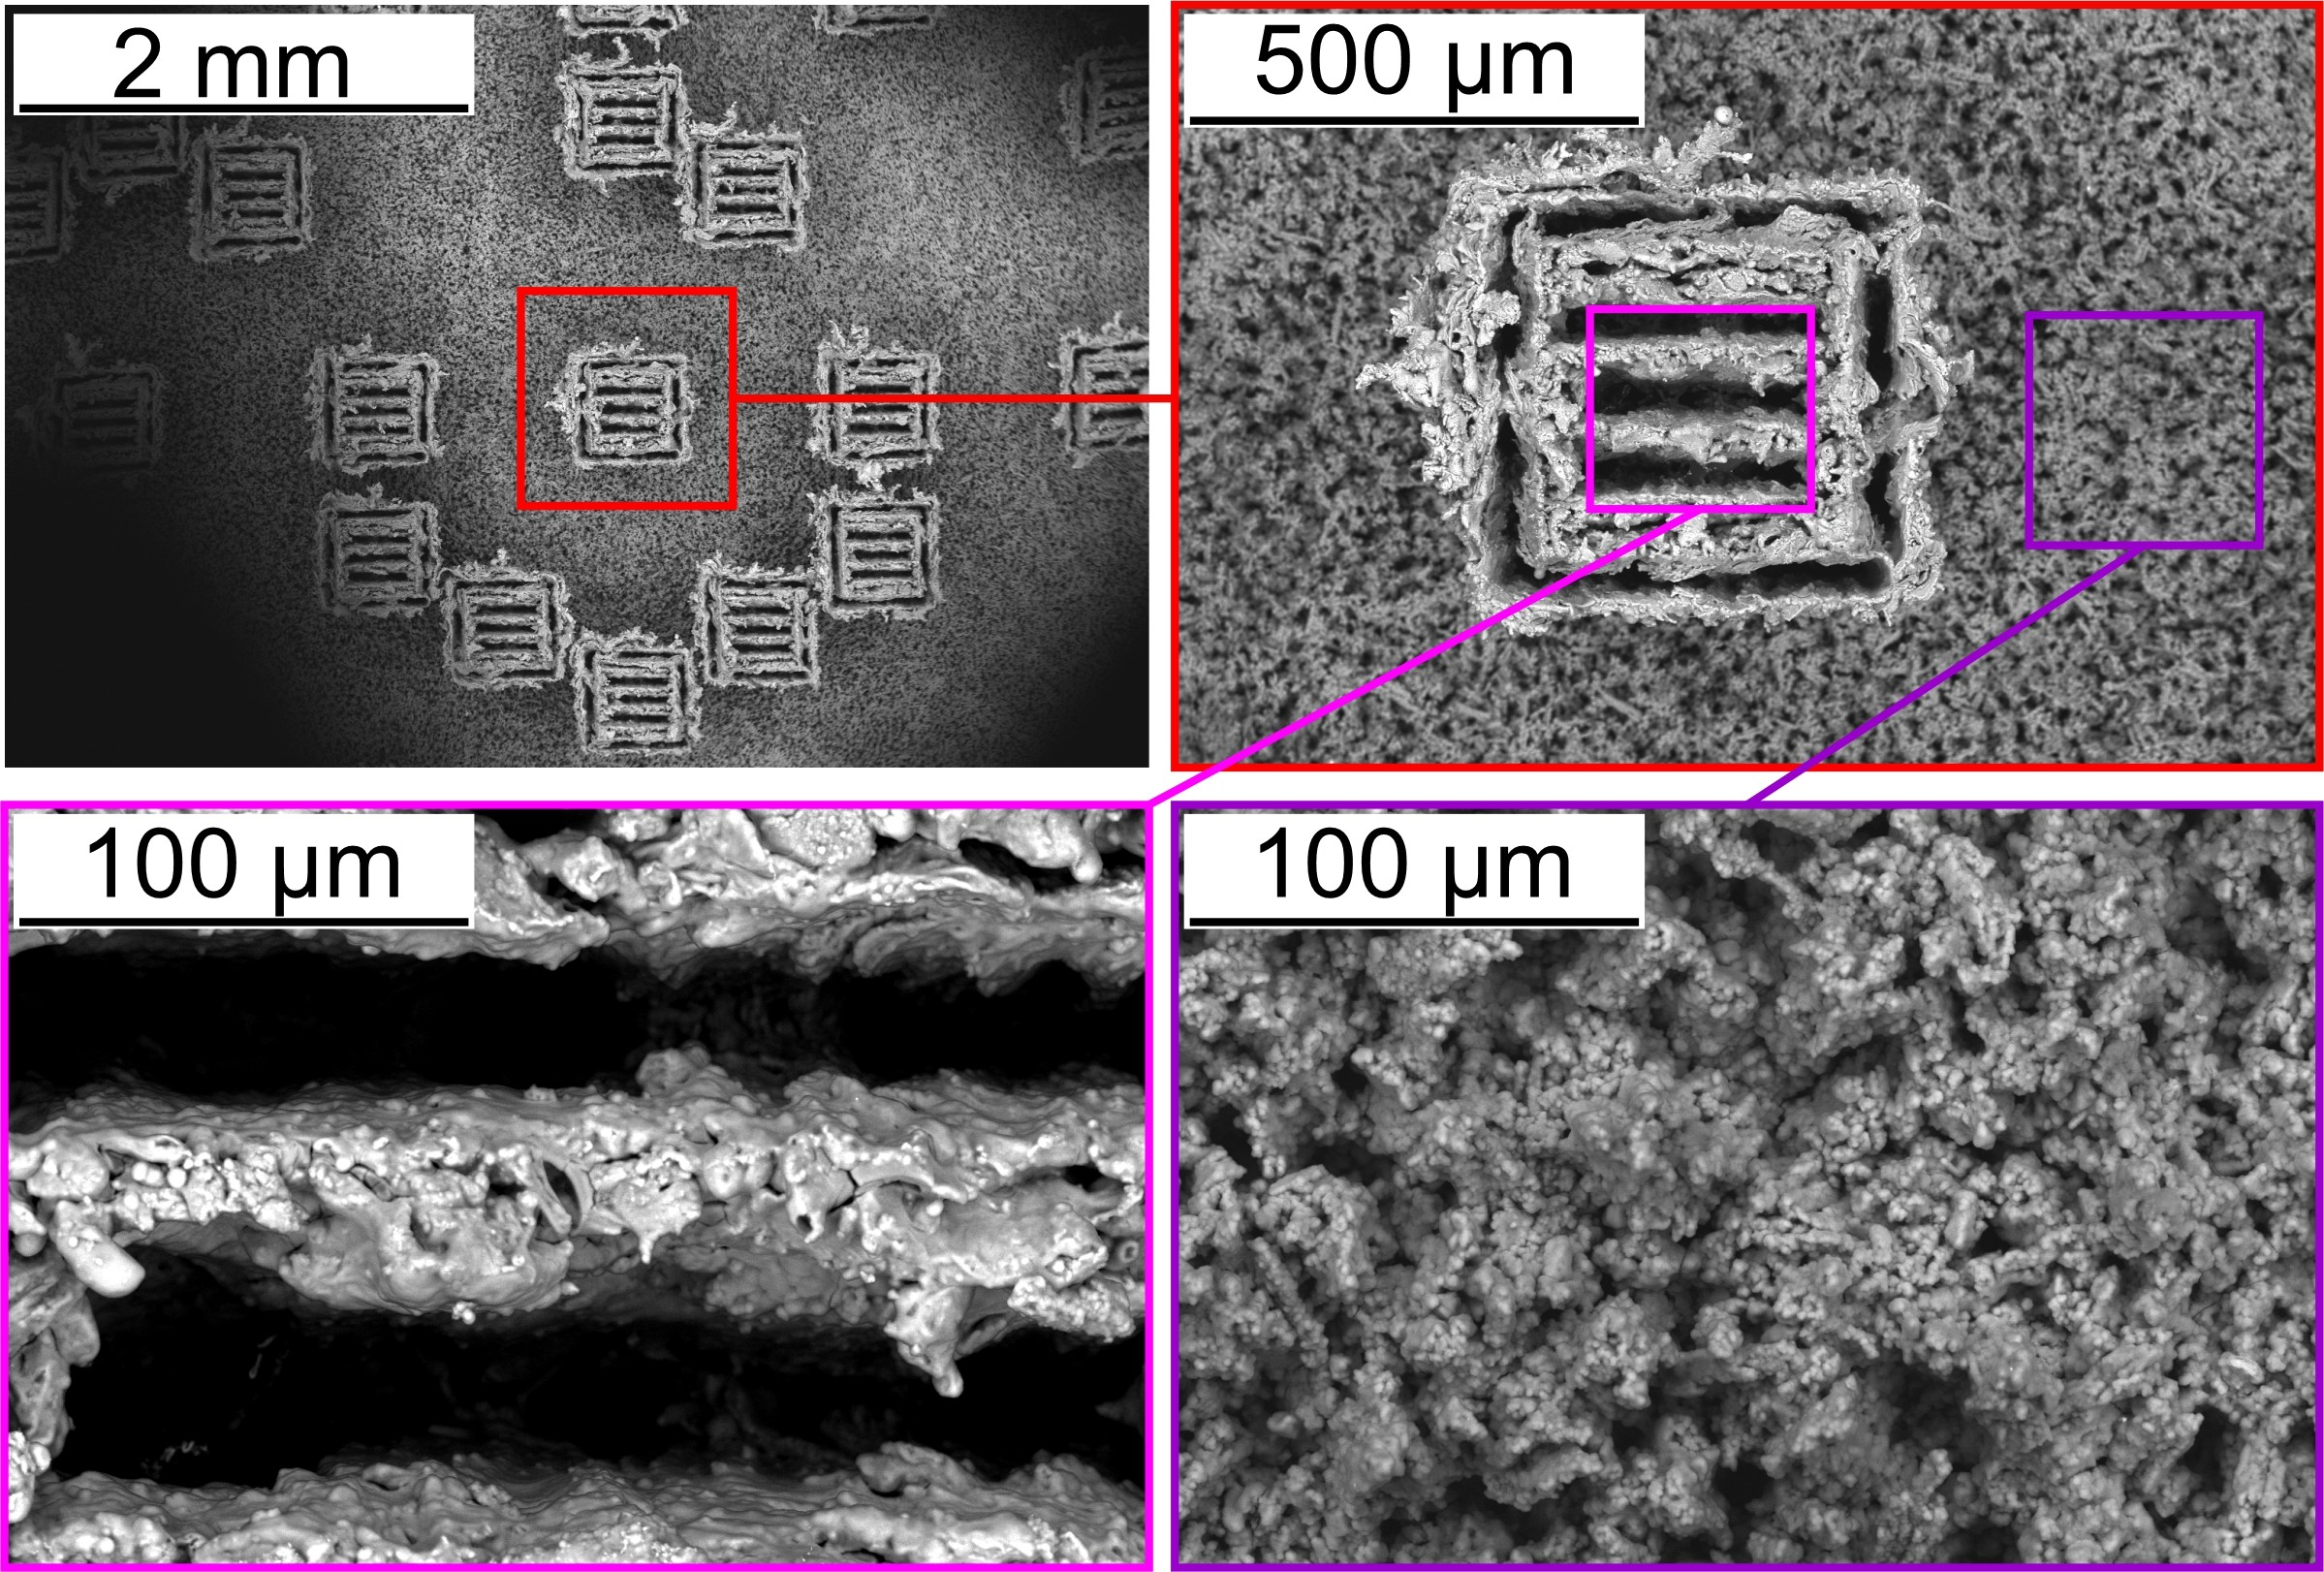
\includegraphics[width=101.5mm]{slike/tekstura.jpg}
	\caption{Lasersko teksturiran in kemično jedkan aluminijev vzorec, posnet z vrstičnim elektronskim mikroskopom \cite{grote2021}.}\label{fig:tekstura}
\end{figure}

Vsaka slika (npr.~slika~\ref{fig:polimerizacija} in slika~\ref{fig:diagrami}) naj bo pred pojavitvijo omenjena v besedilu in tudi širše pojasnjena. Običajno sliko umestimo pod odstavek, v katerem jo prvič omenimo. Če sliko zaradi bolj tekočega oblikovanja besedila umestimo drugače, naj bo umeščena v bližini prve omembe v besedilu, vendar za prvo omembo. Pri sklicevanju na slike in druge dele besedila sledite navodilom, ki so opisana v \textbf{prilogi \ref{cha:priloga}}.

\begin{figure}[htbp]
	\centering
	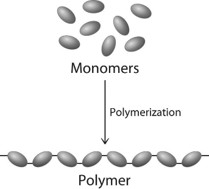
\includegraphics[width=55.2mm]{slike/polimeri.jpg}
	\caption{Shematski prikaz postopka polimerizacije s primerom prevoda tujih izrazov na izvirni sliki v slovenščino \cite{bower2025,stephan2021}.}\label{fig:polimerizacija}
\end{figure}

Če je slika ali del slike povzet iz drugega vira, ga je potrebno citirati, kot je to prikazano na primeru slik \ref{fig:tekstura} in \ref{fig:polimerizacija}. Če je na sliki diagram, morajo biti veličine in enote vseh osi jasno in dosledno označene. Pri razmejevanju naslova osi in enot uporabite enoten stil v celotnem delu (tako na slikah, v enačbah in v besedilu dela). Imenu osi na diagramih naj sledi oznaka veličine in enote, ki jih zapišite v oglatem ali okroglem oklepaju (vseskozi uporabljajte zgolj en način). Primer prikazuje slika \ref{fig:diagrami}.

\begin{figure}[htbp]
	\centering
	\begin{subfigure}[b]{77mm}
		\centering
		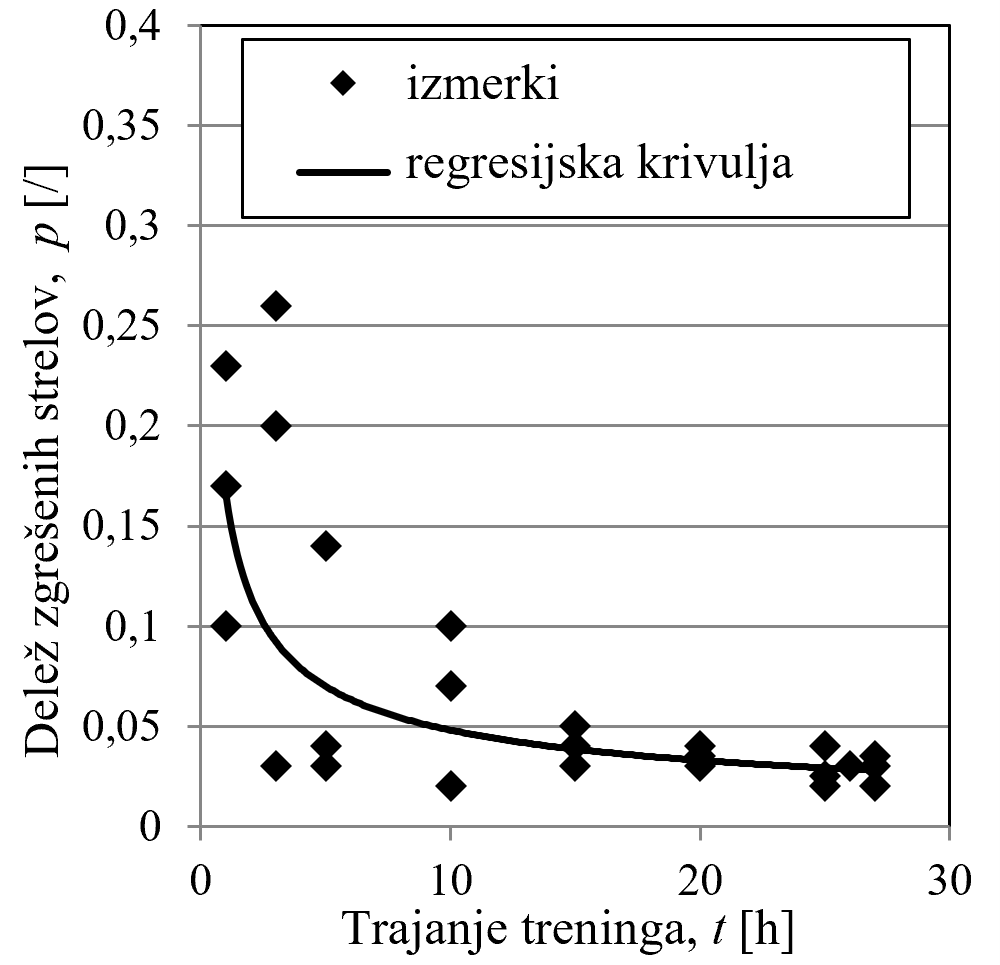
\includegraphics[width=\linewidth]{slike/streli_a.png}
		\caption{}\label{fig:diagrami_a}
	\end{subfigure}\hfill
	\begin{subfigure}[b]{77mm}
		\centering
		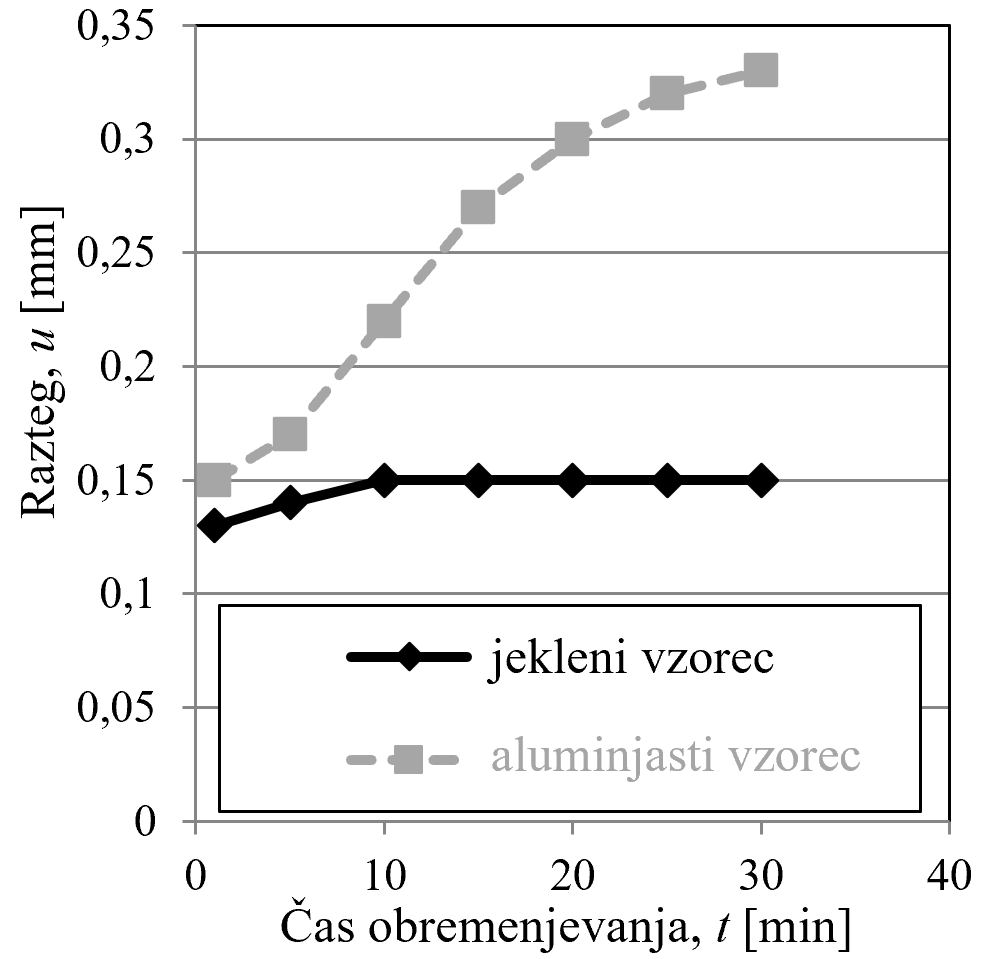
\includegraphics[width=\linewidth]{slike/streli_b.png}
		\caption{}\label{fig:diagrami_b}
	\end{subfigure}
	\caption{(a) Odvisnost deleža zgrešenih strelov na tekmovanju v odvisnosti od časa treninga pred njim. (b) Deformacija v odvisnosti od časa obremenjevanja za dva različna vzorca.}\label{fig:diagrami}
\end{figure}

Na mikroskopskih posnetkih mora biti ustrezno označena dolžinska skala, kot to prikazuje slika \ref{fig:tekstura}. Pri zaporedju časovno razmejenih slik naj bodo označeni relativni časi, kot to prikazuje slika \ref{fig:padec}.

\begin{figure}[htbp]
	\centering
	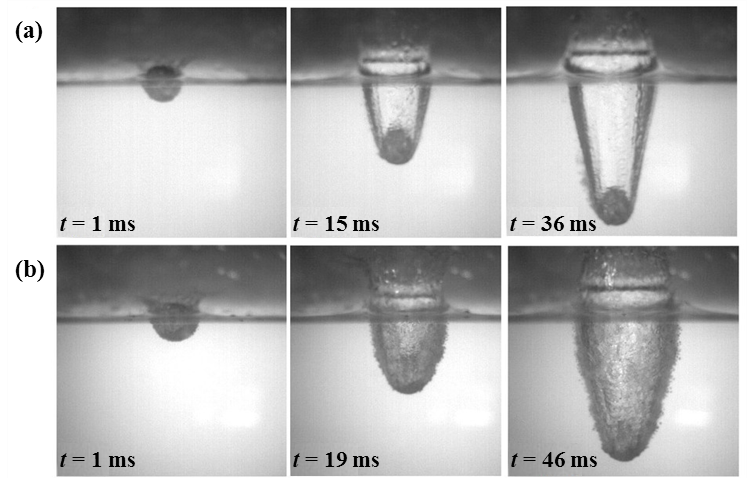
\includegraphics[width=126.5mm]{slike/mikroskop.png}
	\caption{Časovno sosledje padca projektila v vodo z višine (a) 2,1~m; in (b) 4,1~m \cite{tsao1993}.}\label{fig:padec}
\end{figure}

Kot je prikazano na slikah \ref{fig:diagrami} in \ref{fig:padec}, lahko več povezanih delov slike združite v eno sliko, pri čemer jih jasno ločite na podsklope, tj. (a), (b),\ldots{} Pri tem pazite na preglednost. Posamezni podsklopi morajo biti obrazloženi v napisu slike. Pri sklicevanju na posamezen podsklop slike v besedilu dela to storite z navedbo črke v oklepaju takoj za številko slike, npr. slika \ref{fig:padec}(b).

\section{Enačbe}\label{sec:enacbe}
Za vnos enačbe uporabljajte način \verb|equation|. To bo samodejno vstavilo enačbo s samodejnim oštevilčenjem okroglem oklepaju.

Enačbo nato prilagodite in po potrebi posodobite zaporedno številko enačbe v poglavju. Podrobna navodila glede vstavljanja in oblikovnega izgleda enačb so navedena v \textbf{prilogi \ref{cha:priloga}}.

V nadaljevanju so prikazani primeri enačb. Številčenje se začne s številko prve ravni poglavja, v katerem se enačba nahaja, sledi zaporedna številka enačbe v tem poglavju. Pojasnilo enačbe in veličin, ki se v enačbi pojavijo prvič, mora biti v besedilu.

To je primer matematičnega zapisa drugega Newtonovega zakona
\begin{equation}\label{eq:F}
	\bm{F}=m\bm{a},
\end{equation}
kjer so $\bm{F}$ sila, $m$ masa telesa in $\bm{a}$ pospešek telesa. Enačba, ki je vstavljena v poved, se konča z ločilom, če je to potrebno. Enačba, ki stoji samostojno, ločila ne potrebuje. Dve zanimivi enačbi sta:
\begin{equation}\label{eq:e}
	e=mc^2
\end{equation}
in
\begin{equation}\label{eq:ecel}
	e_\mathrm{cel}=\sum_{i=1}^{n} m_i c^2.
\end{equation}
Pri tem je $e$ energija delca, $c$ je svetlobna hitrost in $e_\mathrm{cel}$ je energija celotnega sistema.

V besedilu, če je to potrebno, se sklicuje na ustrezno številko enačbe s celo besedo, npr.~na enačbo \eqref{eq:F}. Navodila za dodajanje sklicev na določena dela besedil ali elementov so opisana v \textbf{prilogi \ref{cha:priloga}}.

\subsection{Oznake veličin}\label{sec:oznake_velicin}
Za oznake veličin in druge simbole običajno uporabljamo črke latinske in grške abecede, včasih z dodatki indeksov in drugih znakov. Kot je prikazano v enačbah \eqref{eq:F}--\eqref{eq:ecel}, morajo biti simboli, torej oznake skalarnih veličin, npr.~$e$ ali $m$, pisane v poševnem tisku, vektorske in tenzorske (matrične) veličine, npr.~sila $\bm{F}$, pa morajo biti pisane v poševnem in krepkem tisku. Pri tem oblikovanju sledite pravilom standarda ISO 80000.

Indekse običajno uporabimo, kadar imata dve veličini enak simbol, ali pa če želimo veličino dodatno opredeliti (npr.~$_\mathrm{dop}$ kot dopustni, $_\mathrm{cel}$ kot celoten, $_\mathrm{z}$ kot začetni itn.). Če so ti indeksi opisni, se pišejo pokonci.

Indekse, ki označujejo fizikalne veličine, pišemo v poševnem tisku, npr.~$c_p$, ki predstavlja specifično toploto pri konstantnem tlaku.

Indeksi, ki opisujejo mesta v zaporedju, v matriki itn., se pišejo poševno. Tak primer je $\bm{F}_i$, kjer to pomeni $i$-to silo ali $\bm{A}_{ij}$, kjer to pomeni element $i$-te vrstice in $j$-tega stolpca v matriki $\bm{A}$.


\section{Citiranje in navajanje virov}\label{sec:citiranje}
Pri citiranju upoštevajte pravila citiranja, ki ne veljajo le za zaključna dela, temveč tudi v splošnem za vsako predstavitev, v kateri sta uporabljeni intelektualna ali materialna lastnina drugih avtorjev. Kot vire v čim večji meri uporabljajte novejšo relevantno mednarodno strokovno literaturo. Spletni viri lahko predstavljajo \textbf{največ 25~\%} vseh virov, uporabljenih v doktorskem delu.

Vso uporabljeno literaturo v besedilu morate navajati sproti po zaporednih številkah v \textbf{oglatem oklepaju}, zato naj bo tudi popis bibliografije oštevilčen v skladu z zaporedjem pojavljanja citatov v dokumentu. Različni primeri ustreznega navajanja literature so prikazani v naslednjem odstavku.

V delu Zhang et al.~\cite{zhang2025} je podan pregled vplivov površinske obdelave na delovanje zobniške dvojice. V prispevku \cite{zhang2025} je podan pregled vplivov površinske obdelave na delovanje zobniške dvojice.

V kolikor se trditev ali informacija, ki jo navajate, nanaša na več virov, je potrebno te navesti znotraj enega oglatega oklepaja. Na primer \cite{grote2021,bower2025}, \cite{grote2021,bower2025,stephan2021,tsao1993} ali \cite{grote2021,stephan2021,zhang2025,zibert2025,niculuta2012,gyroid,dawkins,znidarsic2025,merkur2005,surs2009,zgd1,iso690}. Če uporabljate LaTeX, se združevanje referenc izvede avtomatsko.

Zaporedna številka vira, na katerega se sklicujemo v oglatem oklepaju, se ponovi v popisu literature. Vzorci popisa literature so navedeni v \textbf{prilogi \ref{cha:priloga}}. Pri kasnejšem ponovnem sklicevanju na isto referenco uporabimo enako številko kot pri prvem sklicu.
\chapter{Raziskovalne hipoteze / cilji}\label{cha:hipoteze}
Na tem mestu na podlagi predstavljenega \emph{Pregleda stanja razvoja} povzemite dosedanje ključne izsledke in ugotovitve. Na podlagi tega navedite odprta vprašanja in problematiko, ki do tega trenutka še niso bili razrešeni.

V tem poglavju definirajte raziskovalne hipoteze, ki ste jih postavili ob \emph{Pregledu stanja razvoja} in so vam služile kot izhodišče za zasnovo doktorskega dela.

Namesto raziskovalnih hipotez lahko opredelite raziskovalne cilje. Skladno s tem ustrezno izberite naslov tega poglavja.

\section{Publikacije}\label{sec:publikacije}
V primeru, da so bili rezultati doktorskega dela objavljeni ali pripravljeni kot celovite znanstvene publikacije, lahko v tem podpoglavju navedete seznam objavljenih publikacij. Predstavitev publikacij (seznam) je prostovoljna rubrika.

\chapter{Metodologija raziskav}\label{cha:metodologija}
V tem poglavju glede na tip doktorskega dela (npr.~teoretični ali eksperimentalni) sistematično predstavite, razložite in utemeljite uporabljene metode oz.~postopke (npr.~meritev, izračunov, modelirnih postopkov, predpostavk itn.). Metodologija mora biti opisana dovolj natančno, da je delo ponovljivo.

\chapter{Rezultati}\label{cha:rezultati}
V tem poglavju študent predstavi rezultate meritev, analiz, preračunov in drugih obdelav podatkov, pridobljenih v okviru raziskave. Rezultati naj bodo predstavljeni objektivno.

Običajno je delo obsežnejše in sestavljeno iz več ločenih sklopov, zato najpogosteje rezultate iz posameznega sklopa predstavljate v ločenih (pod)poglavjih. Končna oblika mora biti takšna, da je karseda pregledna, jasna in razumljiva.

Poglavji \ref{cha:rezultati} in \ref{cha:diskusija} lahko združite v enotno poglavje \ref{cha:rezultati} Rezultati in diskusija, v kolikor je za izboljšanje jasnosti in utemeljevanja raziskovalnih hipotez/ciljev to bolj primerno.
% Po potrebi naslov spremenite v »Rezultati in diskusija« in v glavni
% datoteki odstranite \chapter{Diskusija}\label{cha:diskusija}
V tem delu predstavite vaše razumevanje rezultatov, njihovo interpretacijo in morebitne komentarje. Diskusija naj se vseskozi karseda neposredno navezuje na poglavja, ki predstavljajo odprta vprašanja in obravnavano problematiko identificirana v poglavju \ref{cha:pregled} in predstavljene hipoteze/cilje v poglavju \ref{cha:hipoteze}.

Poglavji \ref{cha:rezultati} in \ref{cha:diskusija} lahko združite v enotno poglavje \ref{cha:rezultati} Rezultati in diskusija, v kolikor je za izboljšanje jasnosti in utemeljevanja raziskovalnih hipotez/ciljev to bolj primerno.
.

\chapter{Diskusija}\label{cha:diskusija}
V tem delu predstavite vaše razumevanje rezultatov, njihovo interpretacijo in morebitne komentarje. Diskusija naj se vseskozi karseda neposredno navezuje na poglavja, ki predstavljajo odprta vprašanja in obravnavano problematiko identificirana v poglavju \ref{cha:pregled} in predstavljene hipoteze/cilje v poglavju \ref{cha:hipoteze}.

Poglavji \ref{cha:rezultati} in \ref{cha:diskusija} lahko združite v enotno poglavje \ref{cha:rezultati} Rezultati in diskusija, v kolikor je za izboljšanje jasnosti in utemeljevanja raziskovalnih hipotez/ciljev to bolj primerno.

\chapter{Zaključki}\label{cha:zakljucki}
V tem poglavju najprej koncizno opišite vsebino narejenega dela v okviru raziskav. Zatem po odstavkih ali alinejah napišite bistvene doprinose k znanosti in se jasno opredelite glede dokaza hipotez oz.~izpolnitve zastavljenih ciljev.

\section{Predlogi za nadaljnje delo}\label{sec:nadaljnje_delo}
V posebnem podpoglavju napišite svoje predloge za nadaljnje delo in ostala odprta vprašanja na obravnavanem področju ali morebitnem novo odkritem področju.


\cleardoublepage

\renewcommand{\bibsection}{%
	\chapter*{Literatura}%
	\markboth{Literatura}{}%
	\phantomsection
	\addcontentsline{toc}{chapter}{\protect\brezzamika Literatura}%
	\label{cha:literatura}%
}

\bibliographystyle{FS2026}
\bibliography{References}

% Strani za literaturo nimajo glave, le številko strani (kot v Wordu).
\clearpage
\pagestyle{fancy_nohead}

% Načrt ravnanja z raziskovalnimi podatki je obvezen.
\predpoglavjevkazalu{Načrt ravnanja z raziskovalnimi podatki (NRRP)}\label{cha:nrrp}
Ta priloga je obvezna in jo mora kandidat izpolniti ob predstavitvi rezultatov raziskovalnega dela oziroma ob oddaji doktorske disertacije (ta stavek pred oddajo izbrišite).

\begingroup
\setlist[enumerate]{label=\arabic*.,leftmargin=7.5mm,topsep=2pt,itemsep=12pt,parsep=0pt}
% Vsako polje ima na dnu prostor za odgovor.
\newcommand{\nrrpPolje}[1]{\vspace*{4pt}#1\par\vspace*{12pt}}
\setlength{\tabcolsep}{6pt}
\noindent\begin{tabular}{|>{\setlength{\parskip}{8pt}}p{\dimexpr\textwidth-2\tabcolsep-2\arrayrulewidth\relax}|}
\hline
\nrrpPolje{%
  \textbf{Ime in priimek doktoranda/doktorandke:} \avtor

  \textbf{Doktorski program in področje:} \doktorskiProgram

  \textbf{Naslov doktorske disertacije:} \naslovSlo}\\
\hline
\nrrpPolje{%
  \textbf{Tip podatkov in metode njihovega zbiranja in/ali ustvarjanja}
  \begin{enumerate}
  \item Katere podatke ste zbirali oziroma pridobivali in/ali ustvarjali?
  \item Na kakšen način ste zbirali oziroma pridobivali in/ali ustvarjali nove podatke in kako ste uporabljali že obstoječe za potrebe vaše doktorske disertacije?
  \item Ali ste delali z občutljivimi podatki? Če da, kako ste poskrbeli za etično pridobivanje in/ali ustvarjanje podatkov?
  \end{enumerate}}\\
\hline
\nrrpPolje{%
  \textbf{Način hranjenja in zaščita podatkov med raziskovalnim delom za doktorsko disertacijo}
  \begin{enumerate}
  \item Na kakšen način ste hranili podatke?
  \item Če ste delali z občutljivimi podatki, kako ste skrbeli za njihovo varovanje in zaščito? (v nasprotnem primeru to vprašanje preskočite)
  \end{enumerate}}\\
\hline
\nrrpPolje{%
  \textbf{Dolgotrajna dostopnost in hranjenje podatkov}
  \begin{enumerate}
  \item Kje oziroma v katerem podatkovnem repozitoriju boste hranili podatke na dolgi rok po zaključku raziskovalnega dela in omogočili njihovo dostopnost v skladu z zahtevo 50.~člena Pravilnika o doktorskem študiju UL?
  \item Ali načrtujete za določen čas omejiti dostop do podatkov? Če da, pojasnite razloge (npr.~zaradi zaščite intelektualne lastnine ali patenta, ali navedite drug razlog).
  \end{enumerate}}\\
\hline
\end{tabular}
\endgroup


% Priloge so neobvezne; po potrebi odstranite naslednji vnos.
\priloga{Podrobna navodila za oblikovni izgled zaključnih del na FS}\label{cha:priloga}
% Ukazov, zapisanih z \verb, ni mogoče deliti, zato dovolimo večje presledke.
\setlength{\emergencystretch}{3em}
Priloga ali priloge so lahko dodane le \textbf{izjemoma}. Vsebujejo naj informacije, ki so sicer potrebne za prikaz celovitosti, bi pa motile osnovno poročilo, ker bi bralcu odvračale pozornost od osnovne teme. Sem spadajo npr.~daljša izvajanja enačb, numerični izračuni, ponavljajoči se diagrami, iztiski programov in drugo. Ta dokument vsebuje prilogo, v kateri so predstavljene podrobnosti glede ustrezne uporabe predloge za zaključna dela in navodil za oblikovanje dokumenta, ki se jih je potrebno držati pri izdelavi doktorskega dela.

Kot je razvidno iz te predloge, tako naslov poglavja \textbf{Literatura} kot tudi naslovi morebitnih prilog (npr.~\textbf{Priloga A}) ne smejo biti oštevilčeni, morajo pa biti vključeni v kazalo. Morebitni naslovi na nižjih neoštevilčenih nivojih (npr.~podnaslovi v prilogah) ne smejo biti vključeni v kazalo.

Na koncu dokumenta sta vstavljeni dve popolnoma prazni in neoštevilčeni strani, kar predstavlja prazen vstavljen list, podobno kot na začetku naloge takoj za glavno naslovnico. Gre za list, ki ga vstavijo v tiskarni in je namenjen ustrezni vezavi naloge.

\section*{Urejanje in prevajanje predloge}
V datoteki \texttt{podatki.tex} izpolnite podatke o doktorskem delu, nato uredite izvlečka, zahvalo, sezname in vsebinske datoteke. Glavno datoteko \texttt{predloga.tex} prevajajte z XeLaTeXom in BibTeXom:
\begin{verbatim}
xelatex predloga.tex
bibtex predloga
xelatex predloga.tex
xelatex predloga.tex
\end{verbatim}
Nameščena mora biti pisava Times New Roman. V TeXstudiu nastavite \texttt{predloga.tex} kot glavni dokument in izberite XeLaTeX.

\section*{Formalne strani}
Odločbo o potrjeni temi doktorskega dela shranite kot \texttt{tema.pdf} ob glavno datoteko. Vključijo se vse njene strani. Če datoteke še ni, predloga izpiše nadomestno stran. Zahvalo izključite z ukazom \verb|\zahvalafalse|. Prazno polje \verb|\somentor| izpusti vrstico za somentorja. Številčenje se začne pri notranji naslovnici, izpis številk pa pri zahvali oziroma izvlečku. Uvod se začne na strani~1.

\section*{Uporaba prednastavljenih slogov v predlogi}
Za pisanje doktorskega dela uporabljajte to predlogo, v kateri so že \textbf{prednastavljeni slogi} za poenotenje končne oblike zaključnih nalog na FS. Slogi so nastavljeni v datoteki \texttt{nastavitve.tex}, zato jih ne spreminjajte. 
\section*{Navodila za vstavljanje in oblikovni izgled preglednic}
Preglednice se oštevilčijo samodejno s številko poglavja in zaporedno številko preglednice, ločenima s piko (npr.~2.1). Vsebina preglednic je samodejno izpisana v velikosti 10~pt. Preglednice morajo biti berljive, jasne in pregledne. Pod preglednico ali sliko se lahko z manjšo velikostjo pisave (10~pt ali 8~pt) zapišejo morebitne opombe ali npr.~legenda, kot je prikazano v preglednici~\ref{tab:ucinkovitost}. Na preglednice in slike se sklicujemo v normalnem tisku in z malo začetnico, tako kot v prejšnji povedi. Vse preglednice in slike morajo biti pred njihovo pojavitvijo v delu omenjene v besedilu in tudi širše pojasnjene.

Širina preglednice naj ne presega dovoljene širine besedila na strani. V primeru vstavljanja preglednic, ki presegajo širino 15,5~cm, je potrebno preglednico vstaviti na samostojno stran z ležečo orientacijo. V ta namen preglednico postavite v okolje \verb|landscape| (paket \texttt{pdflscape}), ki preglednico samodejno postavi na novo stran z ležečo usmerjenostjo.

Posamezno preglednico (ali sliko), če je le mogoče, prikažemo na eni strani. Če se zaradi velikosti preglednice ni mogoče izogniti njeni delitvi na več strani, na koncu vsake strani (če se preglednica nadaljuje na naslednji strani) desno spodaj napišemo 'se nadaljuje', na naslednjo stran (kjer se preglednica nadaljuje) levo zgoraj pa 'nadaljevanje'. Na vsaki strani obvezno ponovno natisnemo celotno glavo preglednice, stolpce pa po potrebi oštevilčimo. Za take preglednice uporabite okolje \verb|longtable|; primer ponovljene glave in oznak nadaljevanja je v datoteki \texttt{oznake/oznake.tex}.

Preglednice morajo nujno vsebovati vodoravno obrobo na vrhu in na dnu (ukaza \verb|\toprule| in \verb|\bottomrule| paketa \texttt{booktabs}). Navpične stranske obrobe in notranje obrobe izbrišite, če s tem ni zmanjšana preglednost. Preglednice naj bodo poenotenega videza v celotnem delu in naj ne bodo vstavljene kot slike.

\section*{Navodila za vstavljanje in oblikovni izgled slik}
Slike se oštevilčijo samodejno s številko poglavja in zaporedno številko slike, ločenima s piko (npr.~2.1). Več povezanih delov slike združite v eno sliko z okoljem \verb|subfigure|, kot to prikazuje slika~\ref{fig:diagrami}. 

Slike morajo biti berljive, jasne in pregledne. Slike, ki so preslikane z optičnimi bralniki, naj bodo v čim boljši ločljivosti. Slike, ki jih ustvarjate sami s programi, kot so \emph{Inkscape}, \emph{CorelDraw}, \emph{Photoshop}, \emph{PowerPoint} idr., naj bodo shranjene v vektorskem formatu *.pdf ali izvožene z ločljivostjo 600~dpi v formatu *.png oz.~*.jpg. Na ta način bodo pri pretvarjanju dokumenta v *.pdf obliko ohranjene vse podrobnosti, pri tiskanju pa bo zagotovljena najvišja možna ločljivost. Pri velikosti slik bodite pozorni na količino informacij, ki jo sama slika nosi, in v skladu s tem prilagodite velikost slike (za preproste diagrame ni potrebno, da so razširjeni na polovico strani).

\section*{Navodila za vstavljanje in oblikovni izgled enačb}
Za vnos oštevilčene enačbe uporabite okolje \verb|equation|, takoj za začetkom okolja pa z ukazom \verb|\label{eq:...}| določite oznako za sklicevanje. Enačbe so poravnane 0,5~cm od levega roba besedila, kar je v predlogi že nastavljeno.

Številke enačb se pišejo v okroglem oklepaju na koncu zadnje vrstice, v kateri se enačba nahaja. Številčenje enačbe se začne s številko 1.~ravni poglavja, v katerem se enačba nahaja, druga številka pa predstavlja zaporedno številko enačbe v tem poglavju. Številčenje je samodejno in se ob vstavljanju novih enačb samo posodobi.

\section*{Sklicevanje na dele besedila}
Na slike, preglednice, enačbe in poglavja se sklicujte z ukazom \verb|\ref{...}| oziroma za enačbe z ukazom \verb|\eqref{...}|, ki številko enačbe izpiše v okroglem oklepaju. Oznako elementa, na katerega se sklicujete, določite z ukazom \verb|\label{...}|. Ukaz izpiše le številko, zato besedo pred njo sklanjajte sami in jo s številko povežite z nedeljivim presledkom \verb|~|, npr.~\verb|na sliki~\ref{fig:tekstura}| ali \verb|v enačbi~\eqref{eq:F}|. Na ta način se bodo sklici ohranjali tudi, če boste npr.~v besedilo vrinili nove slike, preglednice ipd.

Podobno se lahko sklicujete tudi na naslove poglavij. Ukaz \verb|\poglavjeref{...}| izpiše številko in naslov poglavja v krepkem tisku, npr.~\poglavjeref{sec:slike}.

\section*{Popis literature}
Popis uporabljene literature mora biti oblikovan v skladu s primeri, ki so navedeni v nadaljevanju. V predlogi popis literature iz podatkov v datoteki \texttt{References.bib} samodejno oblikuje slog \texttt{FS2026.bst}; v oklepaju je naveden ustrezni tip vnosa. Popis literature mora v splošnem obsegati:
\begin{itemize}
\item \textbf{za knjigo ali monografijo} (\verb|@book|):
  \begin{itemize}
  \item Avtor ali urednik: \emph{Naslov knjige}. Izdaja (če obstaja). Založba, kraj, letnica izdaje. DOI (če obstaja)
  \end{itemize}
\item \textbf{za poglavje v knjigi} (\verb|@incollection|):
  \begin{itemize}
  \item Avtor: Naslov poglavja. V: Urednik: \emph{Naslov knjige}. Izdaja (če obstaja). Založba, kraj in letnica izdaje, številka začetne in zadnje strani poglavja. DOI (če obstaja)
  \end{itemize}
\item \textbf{članek v reviji} (\verb|@article|):
  \begin{itemize}
  \item Avtor: Naslov članka. \emph{Ime revije} številka revije (letnica izdaje). DOI (če obstaja)
  \end{itemize}
\item \textbf{prispevek na konferenci} (\verb|@inproceedings|):
  \begin{itemize}
  \item Avtor: Naslov prispevka. V: Urednik: \emph{Naslov zbornika}. Kraj, letnica konference, številka začetne in zadnje strani prispevka (če obstaja). DOI (če obstaja)
  \end{itemize}
\item \textbf{spletne strani} (\verb|@misc| s poljema \verb|url| in \verb|urldate|):
  \begin{itemize}
  \item Avtor (če je naveden): Naslov prispevka. URL: spletna povezava, ogled: datum dostopa
  \end{itemize}
\item \textbf{zaključna dela in doktorske disertacije} (\verb|@phdthesis| oz.~\verb|@mastersthesis|):
  \begin{itemize}
  \item Avtor: \emph{Naslov dela}. Tip dela. Institucija, kraj, leto objave
  \end{itemize}
\end{itemize}

Pri navedbi literature, ki ima več kot dva avtorja ali več kot dva urednika, navedite prva dva avtorja oz.~urednika in zaključite seznam s frazo \emph{et al.} Slog \texttt{FS2026.bst} to naredi samodejno, zato v datoteki \texttt{References.bib} navedite vse avtorje.

Za navajanje virov, kjer oblika ni jasno opredeljena v prejšnjem odstavku, glejte primere vzorcev popisa literature v naslednjem poglavju. Pri tem upoštevajte priporočila standarda SIST ISO 690:2021.

\subsection*{Vzorci popisa literature}
\newenvironment{vzorecreferenc}%
  {\begin{list}{}{\setlength{\leftmargin}{10.5mm}\setlength{\itemindent}{-10.5mm}%
    \setlength{\itemsep}{6pt}\setlength{\parsep}{0pt}\setlength{\topsep}{0pt}}}%
  {\end{list}}

Za knjige:
\begin{vzorecreferenc}
\item K.~H. Grote, H.~Hefazi (ur.): \emph{Springer Handbook of Mechanical Engineering}. Springer, Cham, 2021. DOI: 10.1007/978-3-030-47035-7
\item A.~F. Bower: \emph{Applied Mechanics of Solids}. 2. izdaja. CRC Press, Boca Raton, 2025. DOI: 10.1201/9781003617280
\end{vzorecreferenc}

Za poglavja v knjigi:
\begin{vzorecreferenc}
\item P.~Stephan, F.~Dammel, J.~M. Ochterbeck: Thermodynamics. V: K.~H. Grote, H.~Hefazi (ur.): \emph{Springer Handbook of Mechanical Engineering}. Springer, Cham, 2021, str.~61--128. DOI: 10.1007/978-3-030-47035-7\_3
\end{vzorecreferenc}

Za članke v revijah:
\begin{vzorecreferenc}
\item Y.~H. Tsao, D.~F. Evans \emph{et al.}: Long-Range Attractive Force Between Hydrophobic Surfaces Observed by Atomic Force Microscopy. \emph{Science} 262 (1993). DOI: 10.1126/science.8211182
\item Y.~Zhang, C.~Duan \emph{et al.}: Differential Tooth Surface Modification Method for Reducing Vibration in Spiral Bevel and Hypoid Gears. \emph{Strojniški vestnik -- Journal of Mechanical Engineering} 71 (2025). DOI: 10.5545/sv-jme.2024.1249
\end{vzorecreferenc}

Za konferenčne prispevke:
\begin{vzorecreferenc}
\item K.~Žibert, G.~Turk \emph{et al.}: Eksperimentalna študija tokovnih razmer v modelu človeškega srca s pomožno srčno črpalko. V: B.~Harl, N.~Gubeljak (ur.): \emph{Kuhljevi dnevi 2025}. Ankaran, 2025, str.~142--151
\item M.~C. Niculuţǎ, C.~Veje: Analysis of the thermal behavior of a LiFePO$_4$ battery cell. V: D.~Petit, C.~L. Nilliot (ur.): \emph{6th European Thermal Sciences Conference (Eurotherm 2012)}. Poitiers, 2012. DOI: 10.1088/1742-6596/395/1/012013
\end{vzorecreferenc}

Za spletne vire:
\begin{vzorecreferenc}
\item Gyroid. URL: \url{https://mathworld.wolfram.com/Gyroid.html}, ogled: 23. 12. 2025
\item P.~Dawkins: Conjugate and Modulus. URL: \url{https://tutorial.math.lamar.edu/Extras/ComplexPrimer/ConjugateModulus.aspx}, ogled: 23. 12. 2025
\end{vzorecreferenc}

Za doktorske disertacije in druga zaključna dela:
\begin{vzorecreferenc}
\item A.~Žnidaršič: \emph{Izdelava avtomatiziranega stroja za lupljenje krompirja}. Doktorska disertacija. Fakulteta za strojništvo, Ljubljana, 2025
\end{vzorecreferenc}

Za publikacije organizacij:
\begin{vzorecreferenc}
\item Letno poročilo podjetja Merkur d.d. Kranj. Merkur d.d., Kranj, 2005
\item Statistični letopis Republike Slovenije 2009. Statistični urad Republike Slovenije, Ljubljana, 2009
\end{vzorecreferenc}

Za zakonodajne predpise in standarde:
\begin{vzorecreferenc}
\item Zakon o gospodarskih družbah (ZGD-1). Uradni list RS št. 65/09
\item ISO 690:2021. Information and documentation --- Guidelines for bibliographic references and citations to information resources. International Organization for Standardization, 2021
\end{vzorecreferenc}


\predpoglavjevkazalu{Življenjepis}\label{cha:zivljenjepis}
Tukaj na kratko predstavite svoj življenjepis do zaključka doktorskega dela.


% Zaključni prazen list (dve povsem prazni strani).
\cleardoublepage
\praznastran
\praznastran
\end{document}
